\documentclass{beamer}
\usepackage[T1]{fontenc}
\usepackage[utf8]{inputenc}
\usepackage[cyr]{aeguill}
\usepackage[english]{babel}
\usepackage{amsmath,amssymb,amsthm}
\usepackage{bm}
\usepackage{graphicx}
\usepackage{geometry}
\usepackage{tikz}
\usepackage{diffcoeff}
\usepackage{tcolorbox}
\usepackage{color}
\usepackage{pgffor}

%\usepackage{natbib}

\graphicspath{{./Figures/}}

\mode<presentation> {
	%\usetheme{Singapore}
	\usetheme{Madrid}
}
\usefonttheme{serif}
\usecolortheme{beaver}

\DeclareMathOperator*{\argmax}{arg\,max}
\DeclareMathOperator*{\argmin}{arg\,min}

\newcommand{\matr}[1]{\bm{#1}} 

% make bibliography entries smaller
%\renewcommand\bibfont{\scriptsize}
% If you have more than one page of references, you want to tell beamer
% to put the continuation section label from the second slide onwards
%\setbeamertemplate{frametitle continuation}[from second]
% Now get rid of all the colours
%\setbeamercolor*{bibliography entry title}{fg=black}
%\setbeamercolor*{bibliography entry author}{fg=black}
%\setbeamercolor*{bibliography entry location}{fg=black}
%\setbeamercolor*{bibliography entry note}{fg=black}
% and kill the abominable icon
%\setbeamertemplate{bibliography item}{}


\expandafter\def\expandafter\insertshorttitle\expandafter{%
	\insertshorttitle\hfill%
	\insertframenumber\,/\,\inserttotalframenumber}

%
%\addtobeamertemplate{frametitle}{}{
%	\vskip-1em
%	\begin{tikzpicture}[remember picture,overlay]
%	\node[anchor=north east,yshift=-10pt] at (current page.north east) {
\includegraphics[height=0.8cm]{ISAE-SUPAERO.png}};
%	\end{tikzpicture}
%}

\title[STDplus meeting]{Linear N-port modelling of thin plates}
\author[A. Brugnoli ISAE-SUPAERO ]{\small Andrea Brugnoli \and Francesco Sanfedino \and Daniel Alazard}
%\date{23 janvier 2014}

% Clear the navigation bar
\setbeamertemplate{navigation symbols}{}
%\setbeamercolor{section in head/foot}{fg=black, bg=white} 

\AtBeginSection[]{
	\begin{frame}{Plan}
	\small \tableofcontents[currentsection, currentsubsection]
\end{frame} 
}


\begin{document}
	
\begin{frame}
	\titlepage
\begin{columns}
	\begin{column}{0.5\textwidth}
		\centering
		
\includegraphics[height=0.2\textheight]{ISAE-SUPAERO.PNG}
	\end{column}
	\begin{column}{0.5\textwidth}
		\centering
		
\includegraphics[height=0.2\textheight]{esa_logo.png}
	\end{column}
\end{columns}

\end{frame}

\begin{frame}
\frametitle{Plan}
\small
\tableofcontents
\normalsize
\end{frame}

\section{TITOP model of the Kirchhoff plate }

\begin{frame}{Model Hypothesis}
\begin{tcolorbox}
	\textit{Plane cross sections remains plane and normal to the middle-plane during deformations.} 
	\begin{figure}
		\centering
		\includegraphics[height=0.4\textheight]{Kirchh_sketch.eps}
	\end{figure}	
\end{tcolorbox}

Consequently the displacement field assumes the following expression
\begin{equation*}
u(x,y,z) = -z \diffp{w}{x} \qquad v(x,y,z) = -z \diffp{w}{y} \qquad 
w(x,y,z) = w(x,y)
\end{equation*}
\end{frame}


\begin{frame}{Displacement Field approximation}
General displacement field inside a quadrilateral element (Adini-Clough quadrilateral 1961):
\begin{align*}
w(x,y,t) &= P_{w}(x,y)^T \bm{a}(t) \\
\theta_x(x,y,t) &= \diffp{w}{y} =  P_{\theta_x}(x,y)^T \bm{a}(t) \\
\theta_y(x,y,t) &= -\diffp{w}{x} =  P_{\theta_y}(x,y)^T \bm{a}(t)
\end{align*}
where
\begin{align*}
P_{w}(x,y) &= [1, \; x, \; y, \; x^2, \; xy, \; y^2, \; x^3, \; x^2 y , \; x y^2 , \; y^3 , \; x^3 y , \; x y^3]^T \\
P_{\theta_x}(x,y) &= [0, \; 0, \; 1, \; 0, \; x, \; 2y, \; 0, \; x^2 , \; 2 x y , \; 3y^2 , \; x^3 , \; 3 x y^2]^T \\
P_{\theta_y}(x,y) &= [0, \; -1, \; 0, \; -x, \; -y, \; 0, \; -3 x^2, \; -2 x y , \; y^2 , \; 0 , \; 3 x^2 y , \; y^3]^T \\
\end{align*}

\end{frame}

\begin{frame}{Rigid and Flexible components}
The rigid and flexible part can be split by introducing a parent node (located at ($x_P, y_P$)) containing the rigid vertical displacement ($w_P(t)$) and the linearized rotation along $x$ and $y$ ($\theta_x, \theta_y$)
\begin{equation*}
w(x,y,t) = w_P(t) + \widetilde{y} \theta_x - \widetilde{x} \theta_y + w_f(\widetilde{x}, \widetilde{y}, t)
\end{equation*}
where $\widetilde{x} = x - x_P$ and $\widetilde{y} = y - y_P$

The flexible part is expressed by considering that the constant and linear term of the $P_w(x,y)$ vector are included into the rigid part 
\begin{equation*}
w_f(x,y,t) = P_{w_f}(\widetilde{x}, \widetilde{y})^T \bm{a}_f(t)
\end{equation*}
where
\begin{equation*}
P_{w_f}(\widetilde{x}, \widetilde{y}) = [\widetilde{x}^2, \; \widetilde{x}\widetilde{y}, \; \widetilde{y}^2, \; \widetilde{x}^3, \; \widetilde{x}^2 \widetilde{y} , \; \widetilde{x} \widetilde{y}^2 , \; \widetilde{y}^3 , \; \widetilde{x}^3 \widetilde{y} , \; \widetilde{x} \widetilde{y}^3]^T 
\end{equation*}

Analogously for $\theta_{x, f}$ and $\theta_{y, f}$ 

\end{frame}

\begin{frame}{Nodal Coordinates}

It is now necessary to express $\bm{a}_f(t)$, in term of the nodal coordinates. The 9 components of this vector are found by expressing the flexible coordinates $w_f, \theta_{x, f}$ and $\theta_{y, f}$ at three different corner points. Defining
\begin{equation*}
\begin{aligned}
P_{A_i} &= \begin{bmatrix}
P_{w_f}(\widetilde{x}_{A_i}, \widetilde{y}_{A_i}) &
P_{\theta_{x, f}}(\widetilde{x}_{A_i}, \widetilde{y}_{A_i}) & P_{\theta_{y, f}}(\widetilde{x}_{A_i}, \widetilde{y}_{A_i})
\end{bmatrix}  \\
\bm{q}_{A_i} &= \begin{bmatrix}
w_f(\widetilde{x}_{A_i}, \widetilde{y}_{A_i}) & 
\theta_{x, f}(\widetilde{x}_{A_i}, \widetilde{y}_{A_i}) & \theta_{y, f}(\widetilde{x}_{A_i}, \widetilde{y}_{A_i})  \end{bmatrix}^T 
\end{aligned}  \qquad \forall i=1,\dots,3
\end{equation*}


\begin{columns}
	\begin{column}{0.5\textwidth}
	\centering
	\includegraphics[width=0.8\columnwidth]{Kirchh_elem.eps}	
	\end{column}
	\begin{column}{0.5\textwidth}
		\begin{equation*}
			\bm{a}_f =
			\begin{bmatrix}
			P_{A_1}^T \vspace{1pt}\\
			P_{A_2}^T \vspace{1pt}\\
			P_{A_3}^T \vspace{1pt}\\
			\end{bmatrix}^{-1}
			\begin{pmatrix}
			\bm{q}_{A_1} \vspace{1pt}\\
			\bm{q}_{A_2} \vspace{1pt}\\
			\bm{q}_{A_3} \vspace{1pt}\\
			\end{pmatrix} = P_q^{-1} \bm{q}_f
		\end{equation*}
For a better conditioning of matrix $P_q$ nodes $A_i \; \forall i = 1,2,3$ need to be located as far as possible from $(x_P, y_P)$.
	\end{column}
\end{columns}

\end{frame}

\begin{frame}{Energies}
The kinetic energy is given by
\begin{equation*}
	\mathcal{T} = \frac{1}{2} \int_{0}^{l_x} \int_{0}^{l_y}
	\begin{pmatrix}
	\dot{w}\\
	\dot{\theta}_x\\
	\dot{\theta}_y\\
	\end{pmatrix}^T \begin{bmatrix}
	\rho h & 0 & 0\\
    0 & \frac{\rho h^3}{12} & 0\\
	0 & 0 & \frac{\rho h^3}{12}\\
	\end{bmatrix} \begin{pmatrix}
	\dot{w}\\
	\dot{\theta}_x\\
	\dot{\theta}_y\\
	\end{pmatrix}
	dx dy
\end{equation*}
The elastic energy
\begin{equation*}
\mathcal{K} = \frac{1}{2} \int_{0}^{l_x} \int_{0}^{l_y}
\bm{\kappa}^T \bm{D} \bm{\kappa} 
dx dy
\end{equation*} 
The curvatures and the flexural rigidity matrix are given by
 \begin{equation*}
\bm{\kappa} = \begin{pmatrix}
-\diffp[2]{w_f}{x} \vspace{1pt} \\
-\diffp[2]{w_f}{y} \vspace{1pt} \\
-2 \diffp{w_f}{x,y}  \vspace{1pt} \\
\end{pmatrix}  \qquad 
\bm{D}=\begin{bmatrix}
D & D \nu & 0\\
D \nu & D & 0\\
0 & 0 & \frac{D}{2} (1 - \nu)\\
\end{bmatrix}
\end{equation*}
where $D = \frac{E h^3}{12 (1 - \nu)}$ is the flexural stiffness and $\nu$ is the Poisson ratio.
\end{frame}

\begin{frame}{Mass matrix}
The shape functions for the rigid part are 
\begin{equation*}
	\begin{aligned}
	\bm\phi_{w, r} &= [1, \widetilde{y}, -\widetilde{x}]^T \\
	\bm\phi_{\theta_x, r} &= [0, 1, 0]^T \\
	\bm\phi_{\theta_y, r} &= [0, 0, 1]^T \\
	\end{aligned} \qquad
	\bm\Phi_r = \begin{bmatrix}
	\bm\phi_{w, r}^T \\
	\bm\phi_{\theta_x, r}^T \\
	\bm\phi_{\theta_x, r}^T \\
	\end{bmatrix}
\end{equation*}
For the flexible part 
\begin{equation*}
\begin{aligned}
\bm\phi_{w, f} &= (P_{w, f}^T P_q^{-1})^T \\
\bm\phi_{\theta_x, f} &= (P_{\theta_x, f}^T P_q^{-1})^T \\
\bm\phi_{\theta_y, f} &= (P_{\theta_y, f}^T P_q^{-1})^T \\
\end{aligned} \qquad
\bm\Phi_f = \begin{bmatrix}
\bm\phi_{w, f}^T \\
\bm\phi_{\theta_x, f}^T \\
\bm\phi_{\theta_x, f}^T \\
\end{bmatrix}
\end{equation*}
The Mass matrix takes the form
\begin{equation*}
\bm{M} = 
\begin{bmatrix}
\bm{M}_{rr} & \bm{M}_{rf}\\
\bm{M}_{fr} & \bm{M}_{ff}\\
\end{bmatrix} = 
\int_{0}^{l_x} \int_{0}^{l_y}
\begin{bmatrix}
\bm\Phi_r^T \\
\bm\Phi_f^T \\
\end{bmatrix} \begin{bmatrix}
\rho h & 0 & 0\\
0 & \frac{\rho h^3}{12} & 0\\
0 & 0 & \frac{\rho h^3}{12}\\
\end{bmatrix} \begin{bmatrix}
\bm\Phi_r & \bm\Phi_f \\
\end{bmatrix}
dx dy
\end{equation*}
\end{frame}

\begin{frame}{Stiffness matrix}
	Shape function for the curvatures 
	\begin{equation*}
	\begin{aligned}
	\bm\phi_{\kappa_{xx}} &= \left(-\diffp[2]{P_{w, f}^T}{x} P_q^{-1} \right)^T \\
	\bm\phi_{\kappa_{yy}} &= \left(-\diffp[2]{P_{w, f}^T}{y} P_q^{-1} \right)^T \\
	\bm\phi_{\kappa_{xy}} &= \left(-2 \diffp{P_{w, f}^T}{x,y} P_q^{-1} \right)^T \\
	\end{aligned} \qquad
	\bm\Phi_{\bm{\kappa}} = \begin{bmatrix}
	\bm\phi_{\kappa_{xx}}^T \vspace{1pt} \\
	\bm\phi_{\kappa_{yy}}^T \vspace{1pt} \\
	\bm\phi_{\kappa_{xy}}^T \vspace{1pt} \\
	\end{bmatrix}
	\end{equation*}
	Stiffness matrix
	\begin{equation*}
	\bm{K} = \int_{0}^{l_x} \int_{0}^{l_y}
	\bm\Phi_{\bm{\kappa}}^T \bm{D} \bm\Phi_{\bm{\kappa}}
	dx dy
	\end{equation*}
\end{frame}

\begin{frame}{Work of external forces}
	Calling $F_P^z, T_P^x, T_P^y$ the force and torques that the element is exerting of the parent structure and $F_C^z, T_C^x, T_C^y$ the external force applied at the child node $C$, the work can be evaluated as
	\begin{equation*}
	W_e = \begin{pmatrix}
	w_P \\
	\theta_{x, P} \\
	\theta_{y, P} \\
	\bm{q}_f \\
	\end{pmatrix}^T
	\begin{bmatrix}
	- \bm{I}_{3 \times 3} & \bm{\tau}_{CP}^T \\
	\bm{0}_{n \times 3}   & \bm\Phi_f(\widetilde{x}_C, \widetilde{y}_C)^T	\\
	\end{bmatrix}\begin{pmatrix}
	F_P^z \\
	T_P^x \\
	T_P^y \\
	F_C^z \\
	T_C^x \\
	T_C^y \\
	\end{pmatrix}
	\end{equation*}
	The equations of motions ($\bm{q}_r = (w_P,	\theta_{x}, \theta_{y} )^T$) read
	\begin{equation*}
		\begin{bmatrix}
		\bm{M}_{rr} & \bm{M}_{rf}\\
		\bm{M}_{fr} & \bm{M}_{ff}\\
		\end{bmatrix}
		\begin{pmatrix}
		\ddot{\bm{q}}_{r}\\
		\ddot{\bm{q}}_{f}\\
		\end{pmatrix} + 
		\begin{bmatrix}
		\bm{0}_{3 \times 3} & \bm{0}_{3 \times 9}\\
		\bm{0}_{9 \times 3} & \bm{K}\\
		\end{bmatrix}
		\begin{pmatrix}
		{\bm{q}}_{r}\\
		{\bm{q}}_{f}\\
		\end{pmatrix} = 
		\begin{bmatrix}
		- \bm{I}_{3 \times 3} & \bm{\tau}_{CP}^T \\
		\bm{0}_{n \times 3}   & \bm\Phi_f(\widetilde{x}_C, \widetilde{y}_C)^T	\\
		\end{bmatrix}\begin{pmatrix}
		\bm{F}_P\\
		\bm{F}_C\\
		\end{pmatrix}
	\end{equation*}
\end{frame}

\begin{frame}{Modal coordinates}
The modal coordinates are introduced by solving the eigenvalue problem \begin{equation*}
	\bm{M}_{ff} \bm{V}\bm{\Omega}^2  = \bm{K} \bm{V} \qquad \text{where } \bm{\Omega}^2 = \text{Diag}(\omega_i^2)
\end{equation*}
Applying the transformation $\bm{q} = \bm{V} \bm{\eta}$ the system becomes
\small{
\begin{equation*}
\begin{bmatrix}
\bm{M}_{rr} & \bm{L}_{P}^T\\
\bm{L}_{P} & \bm{I}_{9 \times 9}\\
\end{bmatrix}
\begin{pmatrix}
\ddot{\bm{q}}_{r}\\
\ddot{\bm{\eta}}\\
\end{pmatrix} + 
\begin{bmatrix}
\bm{0}_{3 \times 3} & \bm{0}_{3 \times 9}\\
\bm{0}_{9 \times 3} & \bm{\Omega}^2\\
\end{bmatrix}
\begin{pmatrix}
{\bm{q}}_{r}\\
{\bm{\eta}}\\
\end{pmatrix} = 
\begin{bmatrix}
- \bm{I}_{3 \times 3} & \bm{\tau}_{CP}^T \\
\bm{0}_{n \times 3}   &\bm\Phi_{\eta, C}^T	\\
\end{bmatrix}\begin{pmatrix}
\bm{F}_P\\
\bm{F}_C\\
\end{pmatrix}
\end{equation*}
}
where $\bm{L}_{P} = \bm{V}^T \bm{M}_{fr}$, $\bm\Phi_{\eta} = \bm\Phi_f \bm{V}$ and $\bm\Phi_{\eta, C} = \bm\Phi_{\eta}(\widetilde{x} = x_C - x_P, \widetilde{y} = y_C - y_P)$. Furthermore
\begin{equation*}
	\bm{\tau}_{CP} = \begin{bmatrix}
	1 & y_C-y_P & -(x_C - x_P) \\
	0 & 1 & 0 \\
	0 & 0 & 1 \\ 
	\end{bmatrix}
\end{equation*}
 Damping can be added by introducing matrix $\bm{\Xi}= \text{Diag}(2 \xi_i \omega_i)$.
The acceleration at child node is written as 
\begin{equation*}
	\ddot{\bm{x}}_C = \bm{\tau}_{CP}\ddot{\bm{x}}_P + \bm\Phi_{\eta, C} \bm{\eta}
\end{equation*}
where $\ddot{\bm{x}}_C = \begin{pmatrix}
w_C &\theta_{x, C}&\theta_{y, C} \\
\end{pmatrix}^T$ and $\ddot{\bm{x}}_P = \begin{pmatrix}
w_C &\theta_{x, P}&\theta_{y, P} \\
\end{pmatrix}^T$
\end{frame}

\begin{frame}{2 ports model}
The 2 ports model for the Kirchhoff plate considering as inputs the acceleration at the parent node and the reaction at the child node is the following (see \cite{chebbi:hal-01405184} for a reference on the TITOP method). Given a generic body $\mathcal{L}_i$ the model reads
\footnotesize{
\begin{equation*}
\begin{pmatrix}
\dot{\bm\eta} \\
\ddot{\bm\eta} \\
\hline \ddot{\bm{x}}_C \\
\bm{W}_P \\
\end{pmatrix} = 
\underbrace{\left[
\begin{array}{cc|cc}
\bm{0}_{9 \times 9} & \bm{I}_{9 \times 9} & \bm{0}_{9 \times 6} & \bm{0}_{9 \times 6} \\
-\bm{\Omega}^2 & -\bm{\Xi}  & \bm\Phi_{\eta, C}^T & -\bm{L}_P  \\
\hline
-\bm\Phi_{\eta, C}\bm{\Omega}^2 & -\bm\Phi_{\eta, C}\bm{\Xi} &  \bm\Phi_{\eta, C}  \bm\Phi_{\eta, C}^T & \left(\bm{\tau}_{CP} - \bm\Phi_{\eta, C} \bm{L}_P \right)  \\
\bm{L}_P^T \bm{\Omega}^2 & \bm{L}_P^T \bm{\Xi} &  \left(\bm{\tau}_{CP} - \bm\Phi_{\eta, C} \bm{L}_P \right)^T & \bm{L}_P^T \bm{L}_P - \bm{M}_{rr} \\	
\end{array}
\right]}_{\mathcal{M}_{PC}^{\mathcal{L}_i}}	\begin{pmatrix}
\bm{\eta} \\
\dot{\bm\eta} \\
\hline \bm{W}_C \\
\ddot{\bm{x}}_P \\
\end{pmatrix}
\end{equation*}
}
This model represent the case of a plate clamped at $P$ and free at $C$. Thanks to the fact that the feedthrough matrix has consists of non null terms on the diagonal the inversion of the channel is possible. It is therefore possible to represent other boundary conditions by inversion of the channel. 

\end{frame}

\section{Modes of Kirchhoff plate element}

\begin{frame}{Evaluation of modes}
	Test case for the representation of modes 
	\begin{table}
		\centering
		\begin{tabular}{c|c}
		Coefficient & Numerical value \\
		\hline
		Length along $x$: $l_x [m]$ & 4.143 \\
		Length along $y$: $l_y [m]$ & 2.200 \\
		Thickness: $t [m]$ & 0.04 \\
		Young modulus: $E [GPa]$ & 70 \\
		Poisson Modulus: $\nu [na]$ & 0.35 \\
		Parent node location along $x$: $x_P [m]$ & 0 \\ 
		Parent node location along $y$: $y_P [m]$ & $l_y/2$ \\
		Child node location along $x$: $x_C [m]$ & $l_x$ \\ 
		Child node location along $y$: $y_C [m]$ & $l_y/2$ \\
		\end{tabular}
	\end{table}
\end{frame}

\begin{frame}[allowframebreaks]{Modes}
	\foreach \n in {1,...,9}{
\begin{columns}
	\begin{column}{0.5\textwidth}	
		\begin{figure}[t]
			\centering
			\includegraphics[width=0.95\columnwidth]{Mode_\n.eps}
			\caption{Reduced model}
		\end{figure}	
	\end{column}
	\begin{column}{0.5\textwidth}
		\begin{figure}[b]
			\centering
			\includegraphics[width=0.95\columnwidth]{Mode_\n_mult.eps}
			\caption{Model from \cite{oatao19279} with $20 \times 20$ elements}
		\end{figure}
	\end{column}
\end{columns}
\framebreak
}	

\end{frame}


\begin{frame}{Multiple children}
	Several children can be considered inside this model leading to an N ports model. If two children $C_1, C_2$ are considered
	\tiny{
		\begin{equation*}
		\left[
		\begin{array}{cc|ccc}
		\bm{0}_{9 \times 9} & \bm{I}_{9 \times 9} & \bm{0}_{9 \times 6} & \bm{0}_{9 \times 6} & \bm{0}_{9 \times 6}\\
		-\bm{\Omega}^2 & -\bm{\Xi}  & \bm\Phi_{\eta, C_1}^T & \bm\Phi_{\eta, C_2}^T & -\bm{L}_P  \\
		\hline
		-\bm\Phi_{\eta, C_1}\bm{\Omega}^2 & -\bm\Phi_{\eta, C_1}\bm{\Xi} &  \bm\Phi_{\eta, C_1}  \bm\Phi_{\eta, C_1}^T &  \bm\Phi_{\eta, C_1}  \bm\Phi_{\eta, C_2}^T & \left(\bm{\tau}_{C_1 P} - \bm\Phi_{\eta, C_1} \bm{L}_P \right)  \\
		-\bm\Phi_{\eta, C_2}\bm{\Omega}^2 & -\bm\Phi_{\eta, C_2}\bm{\Xi} &  \bm\Phi_{\eta, C_2}  \bm\Phi_{\eta, C_1}^T &  \bm\Phi_{\eta, C_2}  \bm\Phi_{\eta, C_2}^T  & \left(\bm{\tau}_{C_2 P} - \bm\Phi_{\eta, C_2} \bm{L}_P \right)  \\
		\bm{L}_P^T \bm{\Omega}^2 & \bm{L}_P^T \bm{\Xi} &  \left(\bm{\tau}_{C_1 P} - \bm\Phi_{\eta, C_1} \bm{L}_P \right)^T &  \left(\bm{\tau}_{C_2 P} - \bm\Phi_{\eta, C_2} \bm{L}_P \right)^T & \bm{L}_P^T \bm{L}_P - \bm{M}_{rr} \\	
		\end{array}
		\right]	
		\end{equation*}
	}
\normalsize
The extension to a generic N-ports model is straightforward.
\end{frame}

\section{Modelling of Sentinel Solar Panels}

\begin{frame}{Inversion of channels}
	The feedtrought matrix contains non null this term on the diagonal. This feature makes possible the inversion of whichever input port of the model. Given a generic vector of indexes $\bm{Y}$ the modes whose ports (indexed by $\bm{Y}$) are inverted will be denoted $\left[ \mathcal{M}_{PC}^{\mathcal{L}_i} \right]^{-1\, \bm{Y}}$. \\
	
	By inverting channels the construction of several interconnected panels is possible, like the Sentinel Satellite solar panels
\end{frame}



\begin{frame}{Chain of plates: The Sentinel satellite case}	

\begin{figure}
	\centering
	\includegraphics[width=0.9\textwidth]{Three_panels.eps}
	\caption{Schematic modelisation of the three panels}
\end{figure}
\begin{figure}
	\centering
	\includegraphics[width=0.8\textwidth]{Three_panels_BlockDiagram.eps}
	\caption{Equivalent Block Diagram}
\end{figure}
	
\end{frame}


\begin{frame}{Eigenvalues for the complete model}
	\centering
	\includegraphics[width=0.9\textwidth]{Eigen_3panels.eps}
\end{frame}

\begin{frame}[allowframebreaks]{References}
\footnotesize
\bibliographystyle{unsrt}
\nocite{*}
\bibliography{bibliography_presESA}
\end{frame}

\begin{frame}
\centering
Thank you for your attention. Questions?
\end{frame}
\end{document}
